\documentclass[border=12pt]{standalone}
\usepackage{tikz}
\usetikzlibrary{arrows.meta}

\definecolor{laserbody}{RGB}{40,90,160}
\definecolor{laserbeam}{RGB}{220,60,50}
\definecolor{mirrorsurf}{RGB}{90,110,140}
\definecolor{bsfill}{RGB}{210,230,245}
\definecolor{screenfill}{RGB}{245,235,200}
\definecolor{labelink}{RGB}{30,30,30}

\begin{document}
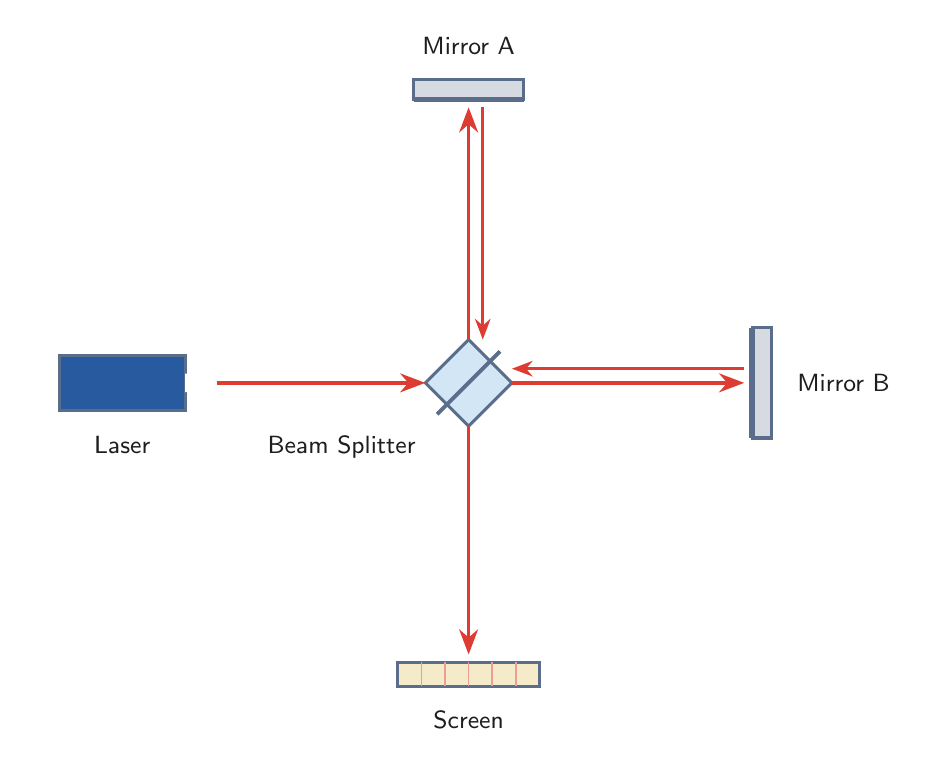
\begin{tikzpicture}[
  >=Stealth,
  component/.style={draw=mirrorsurf, line width=1.1pt},
  beam/.style={draw=laserbeam, line width=1.35pt, ->},
  beamthin/.style={draw=laserbeam, line width=1.0pt, ->},
  lab/.style={font=\sffamily\small, text=labelink},
]

  % Symmetric layout about beam splitter at (0,0)
  % Laser left; Mirror A top; Mirror B right; Screen bottom

  % --- Laser ---
  \draw[component, fill=laserbody] (-5.2,-0.35) rectangle (-3.6,0.35);
  \fill[white] (-3.6,-0.12) -- (-3.25,0) -- (-3.6,0.12) -- cycle;
  \node[lab, below] at (-4.4,-0.55) {Laser};

  % --- Beam Splitter (square rotated 45°) ---
  \draw[component, fill=bsfill]
    (0.55,0) -- (0,0.55) -- (-0.55,0) -- (0,-0.55) -- cycle;
  \draw[mirrorsurf, line width=1.4pt] (-0.4,-0.4) -- (0.4,0.4);
  \node[lab, below left] at (-0.55,-0.55) {Beam Splitter};

  % --- Mirror A (top) ---
  \draw[component, fill=mirrorsurf!25]
    (-0.7,3.6) -- (0.7,3.6) -- (0.7,3.85) -- (-0.7,3.85) -- cycle;
  \draw[mirrorsurf, line width=2pt] (-0.7,3.6) -- (0.7,3.6);
  \node[lab, above] at (0,4.05) {Mirror A};

  % --- Mirror B (right) ---
  \draw[component, fill=mirrorsurf!25]
    (3.6,-0.7) -- (3.85,-0.7) -- (3.85,0.7) -- (3.6,0.7) -- cycle;
  \draw[mirrorsurf, line width=2pt] (3.6,-0.7) -- (3.6,0.7);
  \node[lab, right] at (4.05,0) {Mirror B};

  % --- Screen (bottom) ---
  \draw[component, fill=screenfill]
    (-0.9,-3.85) -- (0.9,-3.85) -- (0.9,-3.55) -- (-0.9,-3.55) -- cycle;
  \foreach \x in {-0.6,-0.3,0,0.3,0.6}
    \draw[laserbeam!50, line width=0.6pt] (\x,-3.55) -- (\x,-3.85);
  \node[lab, below] at (0,-4.05) {Screen};

  % --- Optical paths ---
  % Laser -> BS
  \draw[beam] (-3.2,0) -- (-0.55,0);

  % BS -> Mirror A and return
  \draw[beam] (0,0.55) -- (0,3.5);
  \draw[beamthin] (0.18,3.5) -- (0.18,0.55);

  % BS -> Mirror B and return
  \draw[beam] (0.55,0) -- (3.5,0);
  \draw[beamthin] (3.5,0.18) -- (0.55,0.18);

  % Recombined path to Screen
  \draw[beam] (0,-0.55) -- (0,-3.45);

  % Bounding box ~1200x900 aspect
  \path[use as bounding box] (-5.6,-4.5) rectangle (4.6,4.5);

\end{tikzpicture}
\end{document}
